\chapter{Robust Record-Level Web Extraction Algorithm}
% Describe your own work (how you reached your goal) and take care to motivate your choices. Don't just describe all the things you did – tell us why.

In this chapter, we introduce our algorithm of robust record-level data extraction. We explain the main concepts here and describe them in detail in the following chapter. 

To illustrate the principles, we will use a deliberately simple example and scrape movie titles from an updated web page. Given an innitial web page snapshot with a single movie title marked, we will extract multiple movie titles from an updated snapshot of the same web page. The main steps are depicted in Figure~\ref{fig:algorithm}.

% How each method work. How they are combined.
The main idea of the new method is to split wrapping process into two steps. First, we match the data region boundary. Next, we operate inside the boundary per each data record. We use a minimal tree-edit distance and a probabilistic HTML change model as primary tools for both steps. Eventually, we build a partial tree which is later used for attribute value extraction from multiple data regions. **And pattern matching is used for content double checking.** ???

\begin{figure}[h]
	\centering
	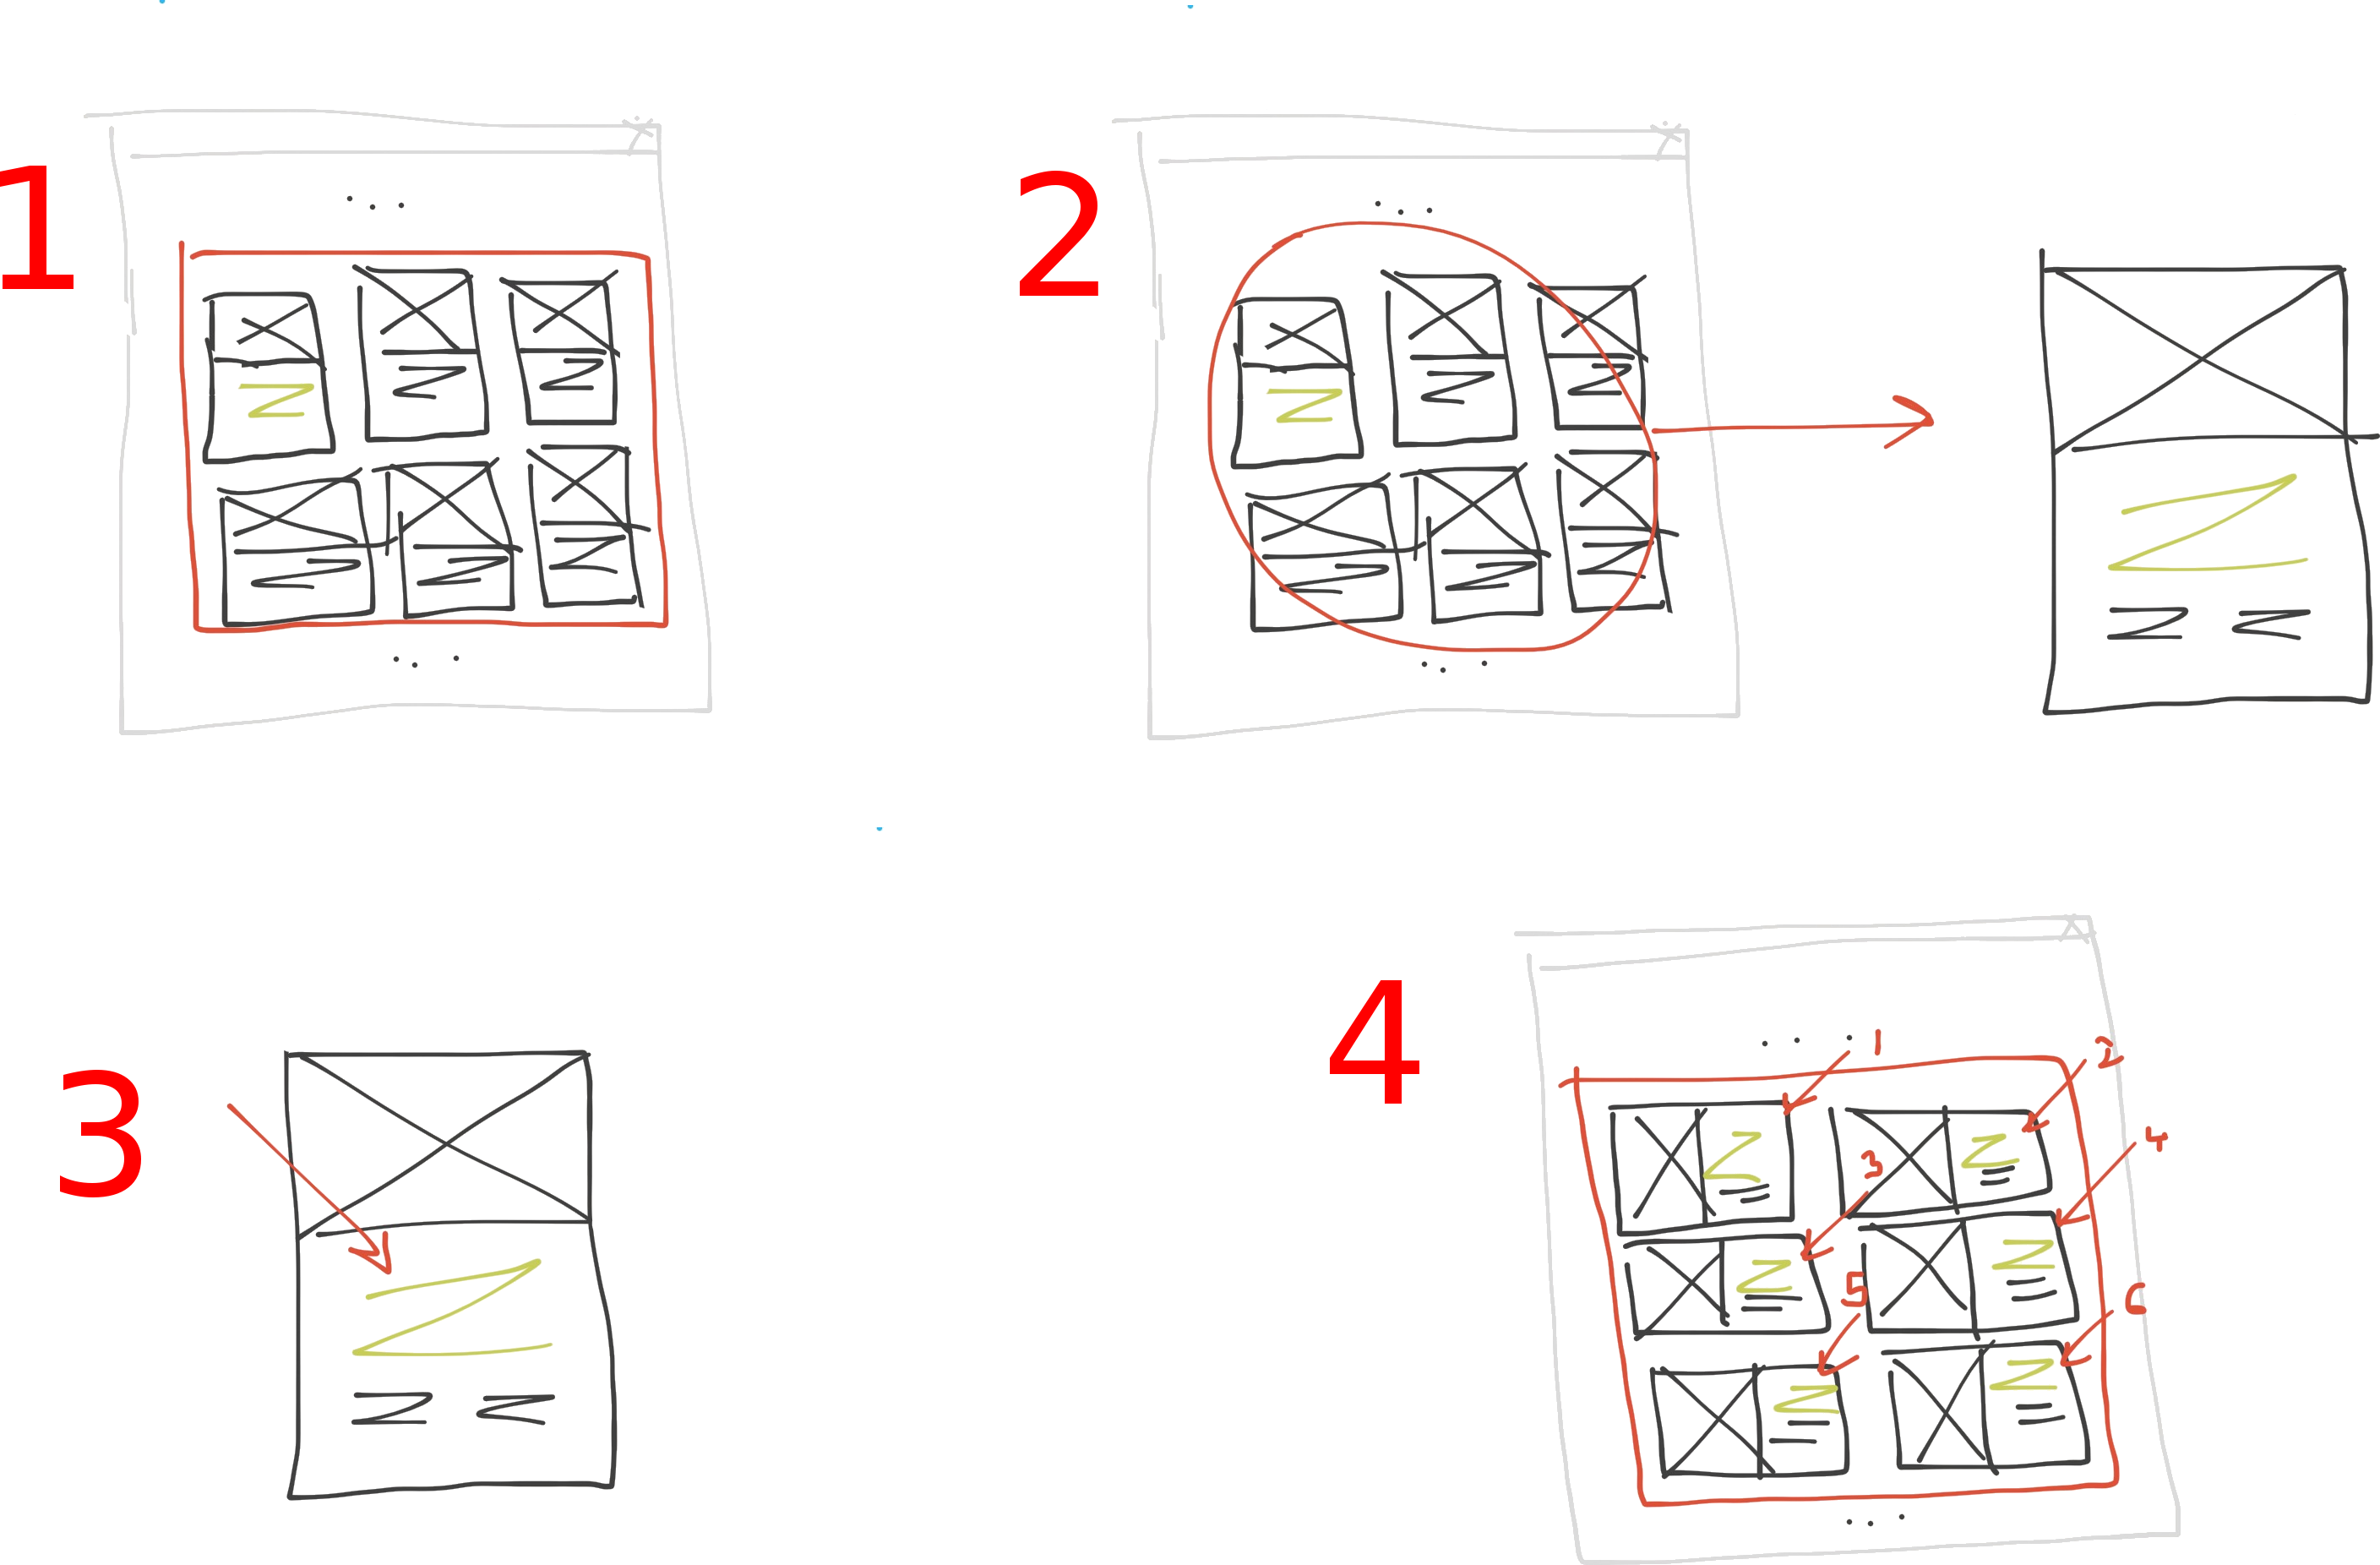
\includegraphics[width=1.0\textwidth]{figures/algorithm}
	\caption{Algorithm steps.}
	\label{fig:algorithm}
\end{figure}

At first, a wrapper is built from original snapshot:

\begin{enumerate}
	\item A global wrapper is built to locate a distinguished node.
	\item Data regions on the original page are located.
	\item A broom is extracted from all regions.
	\item A local wrapper is built for single region.
\end{enumerate}

Finally, wrapping process on the new snapshot takes place:

\begin{enumerate}
	\item A candidate node is located in a new page with a global wrapper.
	\item Data regions on the original page are located.
	\item A local wrapper is run through each data region to extract data records.
\end{enumerate}

% Probabilistic wrapper induction
% TODO Why? Alternatives? 
\cite{DBLP:journals/pvldb/ParameswaranDGR11} introduces the idea of computing edit-distance between two trees, formally defines robustness, and later designs a dynamic programming algorithm for finding the optimal wrapper. Most alternative wrapping techniques [TODO: refs] require large training sets, or use no formal definition of robustness. Yet the method is limited to extracting a single distinguished node from a tree. Thus, we consider it as a state of the art method.

% Data record mining
% TODO Why? Alternatives? 
To enable wrapping in a web page with multiple data records, we need to locate individual data record regions and run page-level wrapper inside a single region. Thus we choose \cite{liu2009a} proposed technique for mining data regions. Unlike most alternatives [TODO: refs] this method ... We also experimented with method variations by implementing tree-edit distance instead of original string edit-distance. And also other optimiztions for our particular use-case.
String matching vs Probabilistic tree change model, which is more accurate

% To illustrate the method in action..
The following example illustrates sample inputs and outputs. An initial snapshot $w_{base}$ of a sample HTML document is illustrated in Figure~\ref{fig:sample-tree}. The annotated attribute node $d(w_{base})$ is marked with parenthesis. The extracted record attribute values are $\{\text{Carol}, \text{Bob}, \text{Alice}\}$.

\begin{figure}[h]
	\centering
	\Tree [.table 
			[.thead 
				[.tr 
					[.th [.\textit{Name} ] ]
					[.th [.\textit{Age} ] ]
				]
			]              
			[.tbody 
				[.tr 
					[.td [.\textit{(Carol)} ] ]
					[.td [.\textit{18} ] ]
				]
				[.tr 
					[.td [.\textit{Bob} ] ]
					[.td [.\textit{19} ] ]
				]
				[.tr 
					[.td [.\textit{Alice} ] ]
					[.td [.\textit{20} ] ]
				]
			]
		]
	\Tree [.table 
			[.tr 
				[.td [.\textit{(Carol)} ] ]
				[.td [.\textit{18} ] ]
			]
			[.tr 
				[.td [.\textit{(Bob)} ] ]
				[.td [.\textit{19} ] ]
			]
			[.tr 
				[.td [.\textit{(Alice)} ] ]
				[.td [.\textit{20} ] ]
			]
		]
	\caption{An initial $w_{base}$ (on the left) and a transformed $w_{new}$ (on the right) snapshots of a sample HTML document. Distinguished nodes marked in paranthesis.}
	\label{fig:sample-tree}
\end{figure}


% ----------------
\section{Framework Overview}

% TODO inputs, outpus, introduce notation and definitions

Inputs: 

\begin{enumerate}
	\item $w_{base}$ -- An initial snapshot of annotated HTML document.
	\item $d(w_{base})$ -- A location of a single record attribute node in the annotated document.
	\item $w_{new}$ -- New (possibly updated) snapshot of the same HTML document.
\end{enumerate}

Outputs: 

\begin{enumerate}
	\item $\{c'_i\}$ -- Extracted attribute values of data records in a new document, e.g. book titles.
	\item $c$ -- \emph{Confidence} measure, i.e. the probability measure that the wrapper did not break. This shows how accurate was the extraction.
\end{enumerate}

\IncMargin{2em}
\begin{algorithm}[h]

	\SetKwFunction{LocateDataRegionContainingNode}{LocateDataRegionContainingNode}
	\SetKwFunction{MergeDataRecords}{MergeDataRecords}
	\SetKwFunction{ProbWrap}{ProbWrap}
	\SetKwFunction{FindRegionContainingNode}{FindRegionContainingNode}
	\DontPrintSemicolon

	\KwData{$w, w', d(w)$}
	\KwResult{$\{c'_i\}$}
	\BlankLine

	$dr$ = \LocateDataRegionContainingNode($w$, $d(w)$) \;
	$r$ = \MergeDataRecords($dr$) \;

	$c'$ = \ProbWrap($w$, $d(w)$, $w'$) \;
	$dr'$ = \LocateDataRegionContainingNode($w'$, $c'$) \;

	\Return $\left\{ \ProbWrap(r, d(w), r') \right\}$, $\forall r' \in dr'$ \;

	\caption{Probabilistic record-level wrapper.}

\end{algorithm}
\DecMargin{2em}

Step 1 of the algorithm on a high-level:

1. Build probabilistic wrapper to locate candidate node in a new tree.\\
2. Build a regional wrapper to locate candidate node inside single record.\\
   - Locate data records in original tree (that contain dist node)\\
   - Build a generic record tree by merging all data records inside original tree.\\
   - Create a regional wrapper for data record wrapping\\

Step 2 of the algorithm:

1. Locate candidate node inside new page.\\
2. Find data regions inside new page (with candidate node).\\
3. Match data records with regional wrapper.\\

% Define the content more carefully: all sections and a brief description what you will write in each of them. Define the main concepts you will need and fix the notations. Then you can write the chapters in any order you want. Make also a work plan: what you will do and when.

% Specify your topic carefully. Don’t take too large topic!  Invent a preliminary title for your thesis and define the content in a coarse level (main chapters). Ask your supervisor’s approval! Decide with your supervisor what material you should read or what experiments to make.  

% You can write the thesis after you have read all material or made all experiments. However, you can begin to write some parts already when you are working. Often you have to change your design plan, but it is just life! Ask feedback from your supervisor, when your work proceeds.

\IncMargin{2em}
\begin{algorithm}
	\KwData{$w, v$}
	\KwResult{$v_{boundary}$}
	\DontPrintSemicolon
	\SetKwFunction{RecordRegions}{RecordRegions}
	\BlankLine

	\For{$v_i \in siblings(v)$}{
		ref [Liu'03]
	}

	\caption{Finding region boundary}
\end{algorithm}
\DecMargin{2em}

\section{Locating Data Region Containing Node}
\section{Merging Data Records}
\section{Probabilistic Wrapping}

% vim: set wrap
